
\labday{Mardi, 04-05-2016}

Expérimentation sur le correcteur. Je vais résumé ici mes résultats et remarques
sur l'utilisation d'un correcteur simple (une seule couche) pour apprendre par l'exemple
à inverser des transformations linéaires simples.

Pour ce j'utilise le modèle simpliste (figure \ref{fig:correcteur}). 
Sans utilisation d'adversarial.

\begin{figure}[H] % Example of including images
\centering
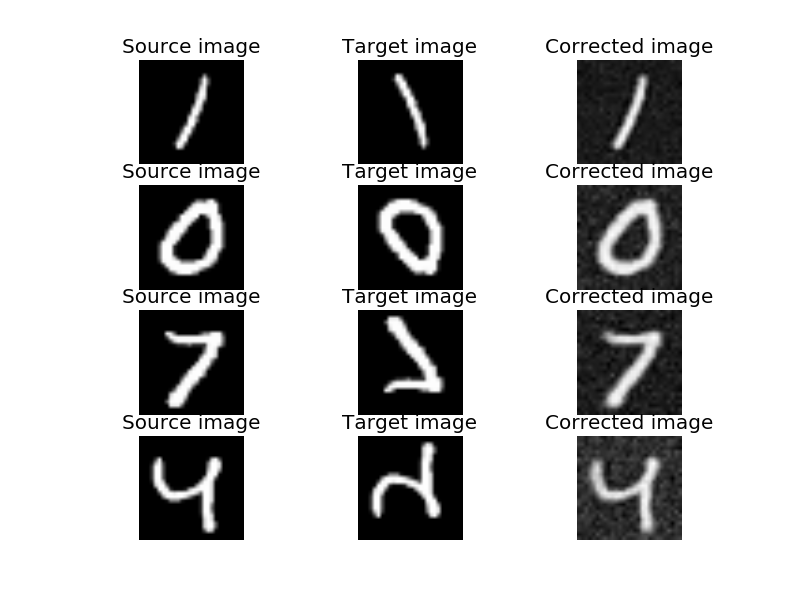
\includegraphics[width=0.45\linewidth]{fig/05-04-2016/MNISTMirror-PairWiseCorrector-lambda-0.0000-sample.png}
\caption{Correcteur simple}
\label{fig:correcteur}
\end{figure}


\experiment{Corriger MNIST après transformations linéaires}

Dans un premier temps sur MNIST.
Le réseaux doit reconstruire l'image transformée.
MNIST est assez pratique car il permet de visualiser facilement l'efficacité 
de la reconstruction pour des données avec un bon nombre de descripteurs (748 pixels).

\subexperiment{Alignées}

Tout d'abord j'ai gardé la correspondance entre l'image original et
l'image transformée pendant l'entraînement du correcteur (cas aligné).
Ainsi chaque paire d'exemple $(x, \phi(x)) \in MNIST\times \phi(MNIST)$
contient uniquement l'information que l'on cherche $\phi$

Ce qui donne de très bon résultats en général.


{\Large\bf Mirror}

\begin{figure}[H] % Example of including images
\centering
\subfigure[Sample images]
	{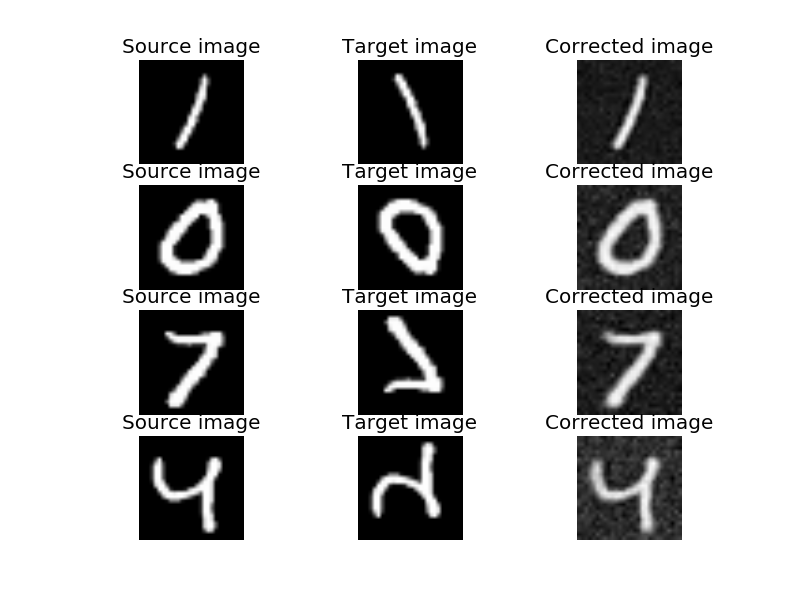
\includegraphics[width=0.45\linewidth]{fig/05-04-2016/MNISTMirror-PairWiseCorrector-lambda-0.0000-sample.png}}
\hfill
\subfigure[Learning curve (squared loss)]
	{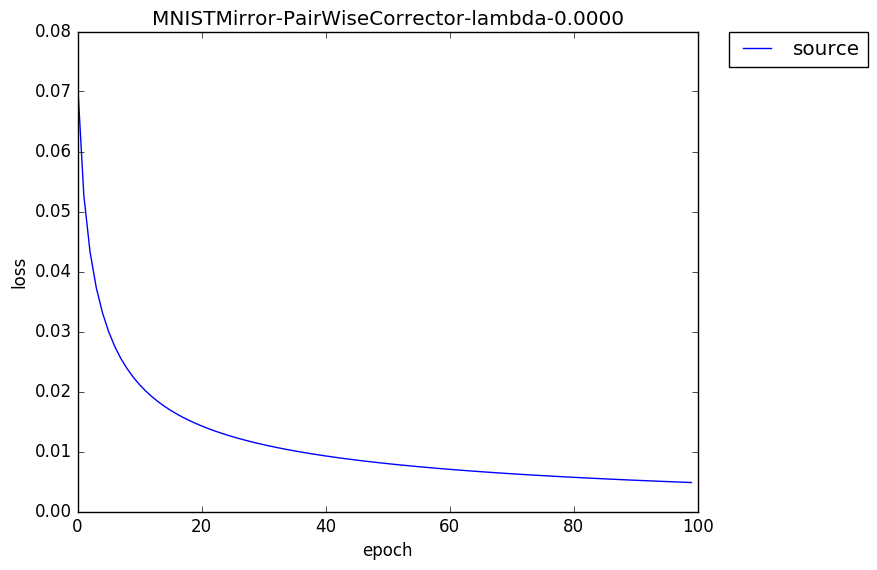
\includegraphics[width=0.45\linewidth]{fig/05-04-2016/MNISTMirror-PairWiseCorrector-lambda-0.0000.png}}
\subfigure[Weights]
	{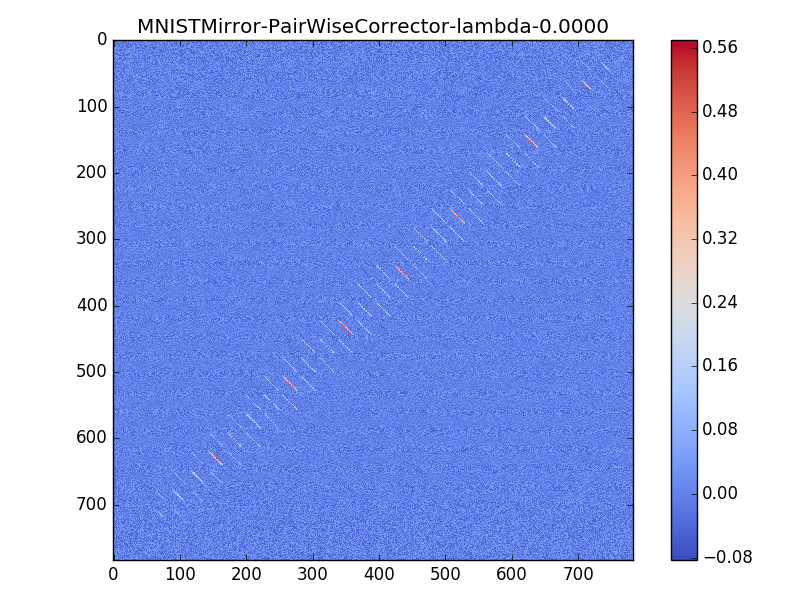
\includegraphics[width=0.45\linewidth]{fig/05-04-2016/MNISTMirror-PairWiseCorrector-lambda-0.0000-Weights.png}}
\caption{MNIST - Mirror correcteur aligné}
\label{fig:mnist_mirror_pairwise}
\end{figure}


{\Large\bf RMat}

\begin{figure}[H] % Example of including images
\centering
\subfigure[Sample images]
	{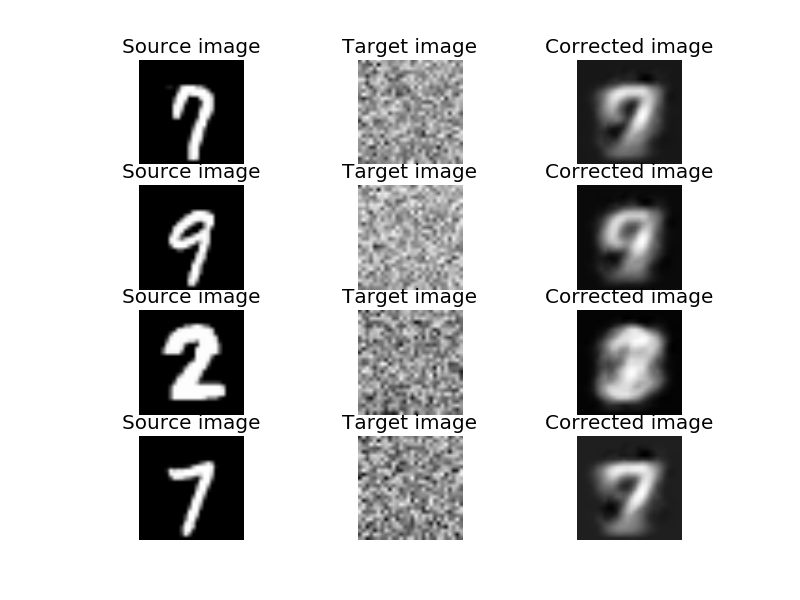
\includegraphics[width=0.45\linewidth]{fig/05-04-2016/MNISTRMat-PairWiseCorrector-lambda-0.0000-sample.png}}
\hfill
\subfigure[Learning curve (squared loss)]
	{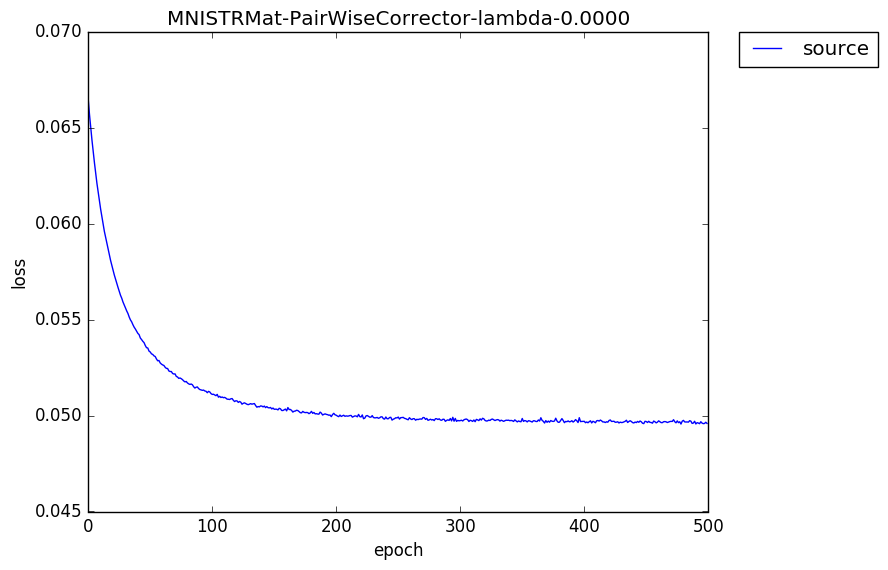
\includegraphics[width=0.45\linewidth]{fig/05-04-2016/MNISTRMat-PairWiseCorrector-lambda-0.0000.png}}
\subfigure[Weights]
	{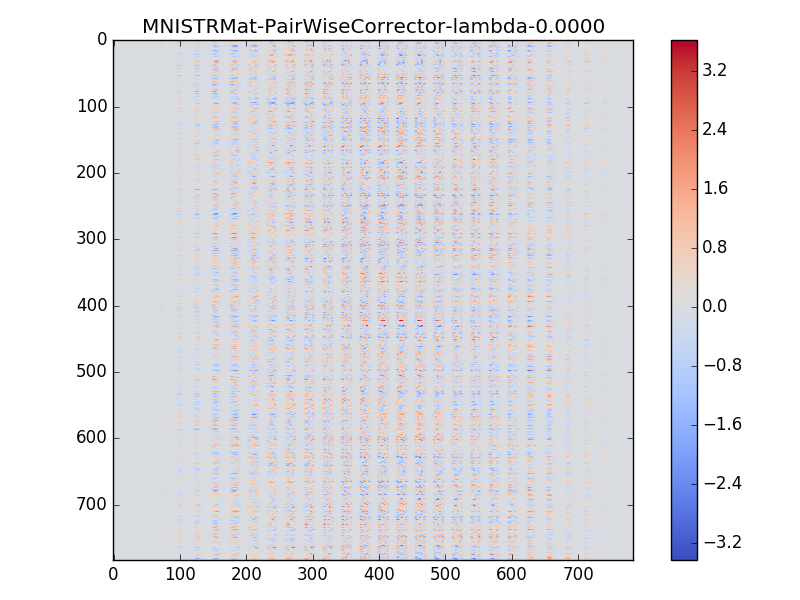
\includegraphics[width=0.45\linewidth]{fig/05-04-2016/MNISTRMat-PairWiseCorrector-lambda-0.0000-Weights.png}}
\caption{MNIST - RMat correcteur aligné}
\label{fig:mnist_rmat_pairwise}
\end{figure}


\subexperiment{Non alignées}

Ici chaque paire d'exemple $(x_i, \phi(x_j)) \in MNIST\times \phi(MNIST)$
ne contient pas uniquement l'information que l'on cherche $\phi$. Même si
les exemples $x_i$ et $x_j$ sont choisis parmi la même classe, ces exemples 
se différencient non seulement par la transformation subie mais aussi par 
les variations au sein d'une même classes.

Ceci est plus proche de cas d'expériences réels. Exemple: des échantillons
du même type sans être exactement les mêmes et utilisant des instruments
de précision différents.

{\Large\bf Mirror}

\begin{figure}[H] % Example of including images
\centering
\subfigure[Sample images]
	{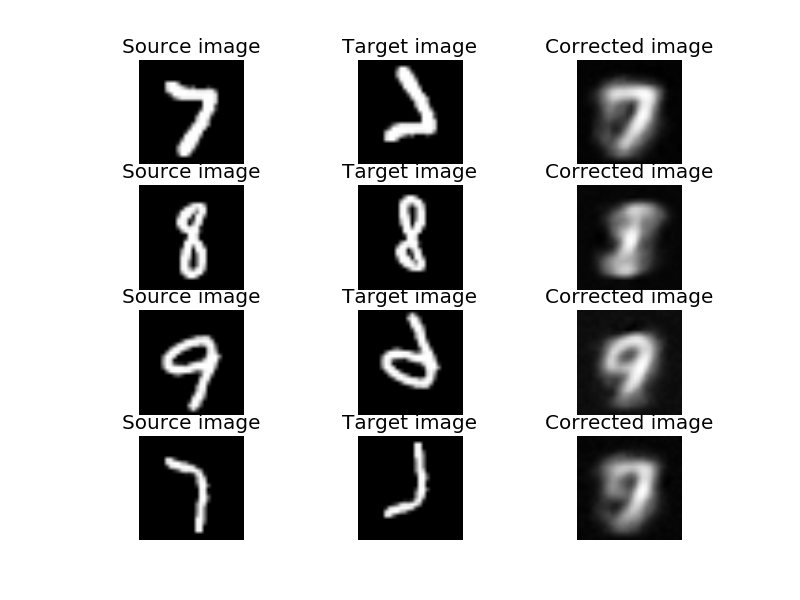
\includegraphics[width=0.45\linewidth]{fig/05-04-2016/MNISTMirror-ClassWiseCorrector-lambda-0.0000-sample.png}}
\hfill
\subfigure[Learning curve (squared loss)]
	{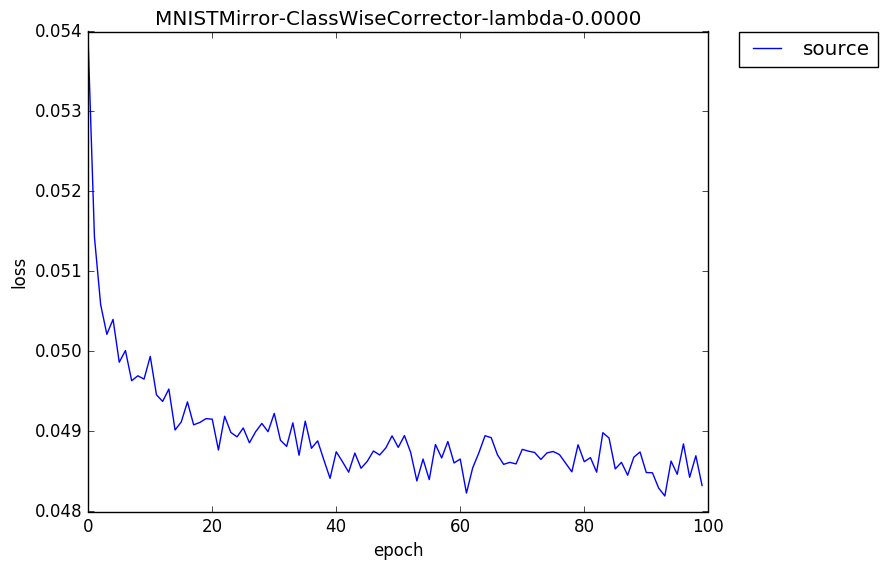
\includegraphics[width=0.45\linewidth]{fig/05-04-2016/MNISTMirror-ClassWiseCorrector-lambda-0.0000.png}}
\subfigure[Weights]
	{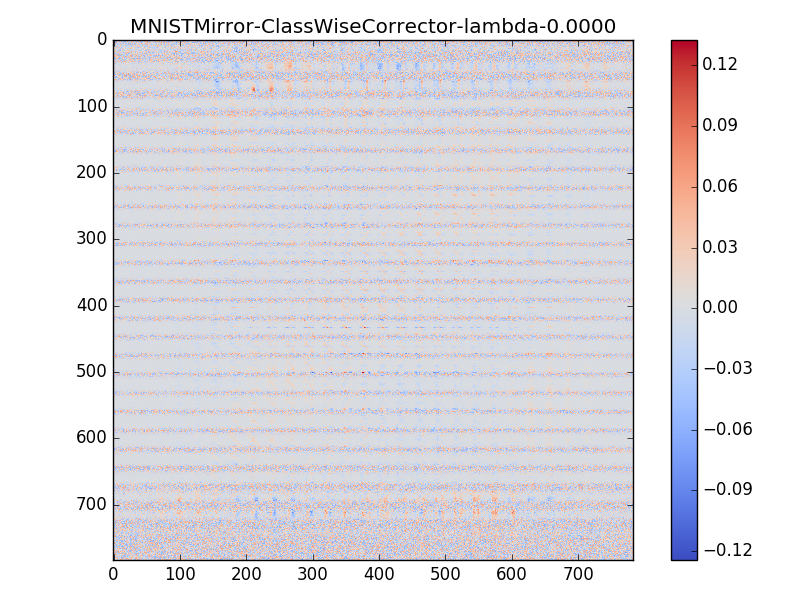
\includegraphics[width=0.45\linewidth]{fig/05-04-2016/MNISTMirror-ClassWiseCorrector-lambda-0.0000-Weights.png}}
\caption{MNIST - Mirror correcteur non aligné}
\label{fig:mnist_mirror_classwise}
\end{figure}


{\Large\bf RMat}

\begin{figure}[H] % Example of including images
\centering
\subfigure[Sample images]
	{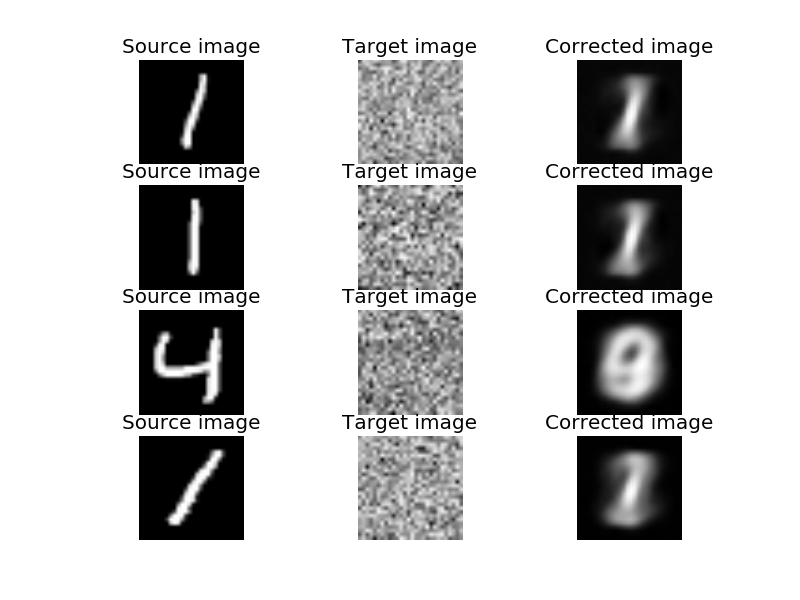
\includegraphics[width=0.45\linewidth]{fig/05-04-2016/MNISTRMat-ClassWiseCorrector-lambda-0.0000-sample.png}}
\hfill
\subfigure[Learning curve (squared loss)]
	{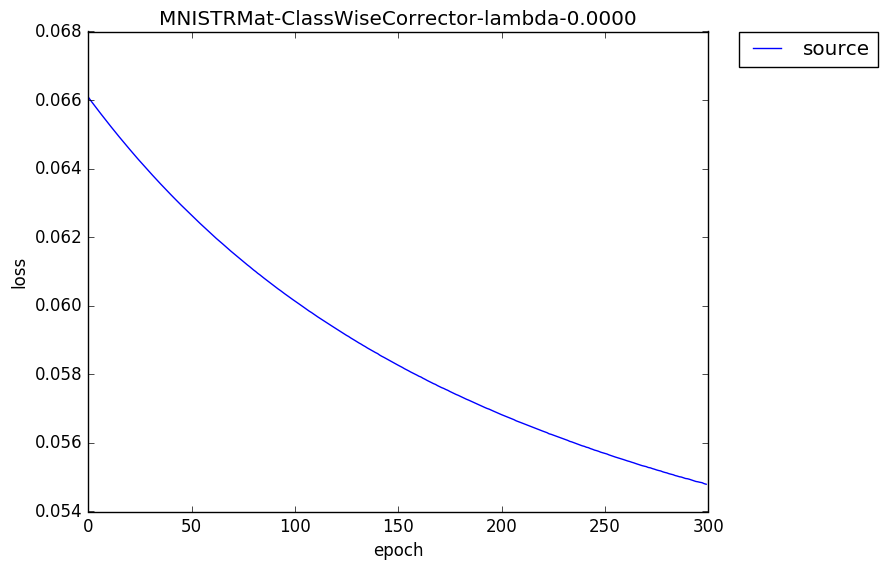
\includegraphics[width=0.45\linewidth]{fig/05-04-2016/MNISTRMat-ClassWiseCorrector-lambda-0.0000.png}}
\subfigure[Weights]
	{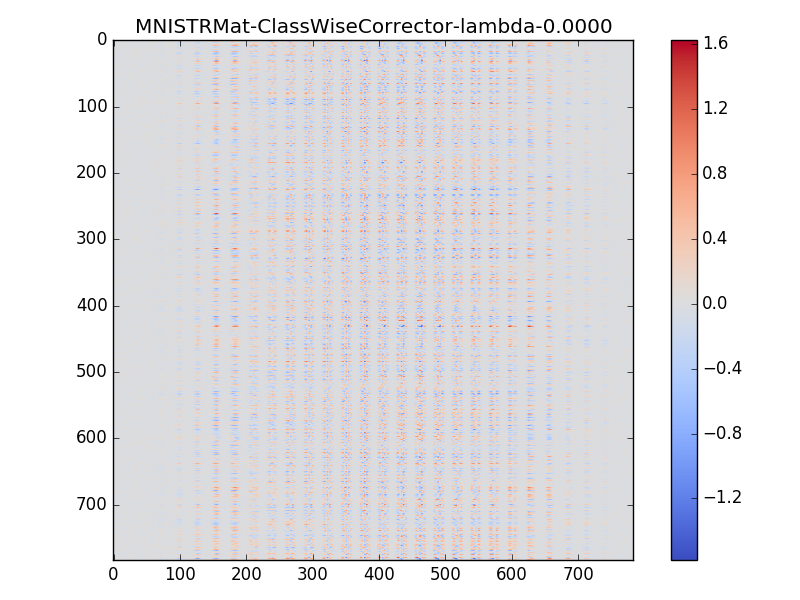
\includegraphics[width=0.45\linewidth]{fig/05-04-2016/MNISTRMat-ClassWiseCorrector-lambda-0.0000-Weights.png}}
\caption{MNIST - RMat correcteur non aligné}
\label{fig:mnist_rmat_classwise}
\end{figure}


%-----------------------------------------

\experiment{Corriger Moon après transformations linéaire}



\begin{table}[H]
\begin{tabular}{l l l}
\toprule
\textbf{Groups} & \textbf{Treatment X} & \textbf{Treatment Y} \\
\toprule
1 & 0.2 & 0.8\\
2 & 0.17 & 0.7\\
3 & 0.24 & 0.75\\
4 & 0.68 & 0.3\\
\bottomrule
\end{tabular}
\caption{The effects of treatments X and Y on the four groups studied.}
\label{tab:treatments_xy}
\end{table}


%----------------------------------------------------------------------------------------
